% Build into figs/ from the repo root: pdflatex -output-directory=figs code/fig_fourcorner.tex && rm figs/fig_fourcorner.aux figs/fig_fourcorner.log
\documentclass[border=4pt]{standalone}
\usepackage[T1]{fontenc}
\usepackage{amsmath,amssymb}
\usepackage[none]{hyphenat}
\usepackage{tikz}
\usetikzlibrary{positioning,arrows.meta,calc}
\definecolor{navy}{HTML}{26456E}
\definecolor{teal}{HTML}{2A8F82}
\definecolor{gold}{HTML}{B8860B}
\definecolor{plum}{HTML}{7B5EA7}
\definecolor{rust}{HTML}{C0562F}
\definecolor{gray}{HTML}{6B6B6B}
\begin{document}
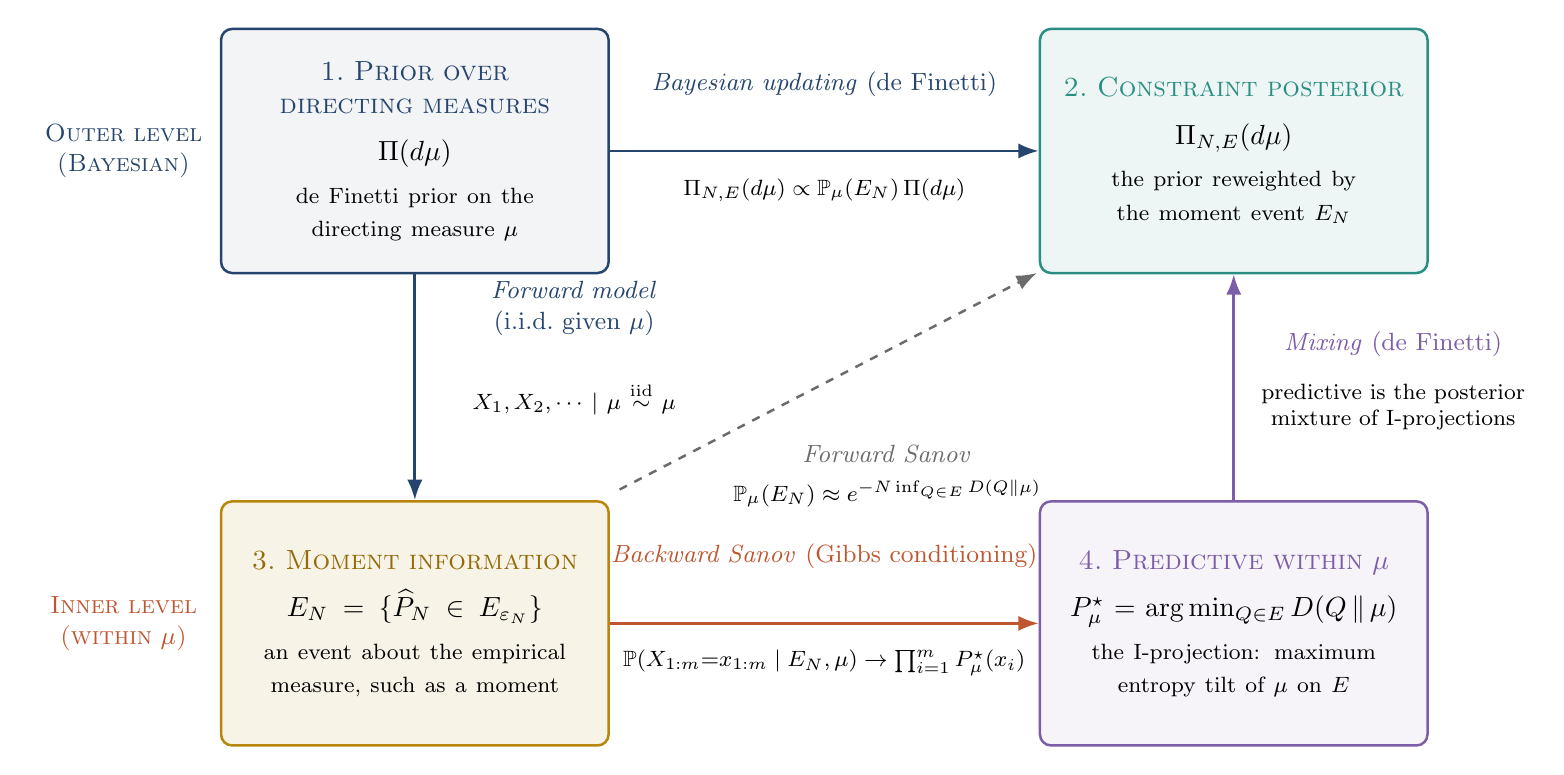
\begin{tikzpicture}[
  cbox/.style={rounded corners=4pt, draw, line width=0.9pt, inner sep=6pt, align=center, minimum height=3.1cm, text width=4.5cm},
  arr/.style={-{Latex[length=2.6mm]}, line width=1pt},
  lab/.style={align=center, font=\small},
  flab/.style={align=center, font=\footnotesize},
]
\node[cbox, draw=navy, fill=navy!6] (b1) at (0,6.0)
  {{\scshape\color{navy} 1.\ Prior over\\ directing measures}\\[5pt] $\Pi(d\mu)$\\[6pt]
   {\footnotesize de Finetti prior on the\\ directing measure $\mu$}};
\node[cbox, draw=teal, fill=teal!8] (b2) at (10.4,6.0)
  {{\scshape\color{teal} 2.\ Constraint posterior}\\[5pt] $\Pi_{N,E}(d\mu)$\\[6pt]
   {\footnotesize the prior reweighted by\\ the moment event $E_N$}};
\node[cbox, draw=gold, fill=gold!10] (b3) at (0,0)
  {{\scshape\color{gold!80!black} 3.\ Moment information}\\[5pt] $E_N=\{\widehat P_N\in E_{\varepsilon_N}\}$\\[6pt]
   {\footnotesize an event about the empirical\\ measure, such as a moment}};
\node[cbox, draw=plum, fill=plum!7] (b4) at (10.4,0)
  {{\scshape\color{plum} 4.\ Predictive within $\mu$}\\[5pt] $P^\star_\mu=\arg\min_{Q\in E} D(Q\,\|\,\mu)$\\[6pt]
   {\footnotesize the I-projection: maximum\\ entropy tilt of $\mu$ on $E$}};
\node[lab, color=navy, text width=2.2cm] at (-3.7,6.0) {\scshape Outer level\\ (Bayesian)};
\node[lab, color=rust, text width=2.2cm] at (-3.7,0) {\scshape Inner level\\ (within $\mu$)};
\draw[arr, color=navy] (b1.east) -- (b2.west);
\node[lab, color=navy] at (5.2,6.85) {\emph{Bayesian updating} (de Finetti)};
\node[flab] at (5.2,5.5) {$\Pi_{N,E}(d\mu)\propto \mathbb{P}_\mu(E_N)\,\Pi(d\mu)$};
\draw[arr, color=navy] (b1.south) -- (b3.north);
\node[lab, color=navy, anchor=west, text width=3.0cm] at (0.4,4.0) {\emph{Forward model}\\(i.i.d.\ given $\mu$)};
\node[flab, anchor=west, text width=3.0cm] at (0.4,2.85) {$X_1,X_2,\dots\mid\mu \overset{\mathrm{iid}}{\sim}\mu$};
\draw[arr, color=rust] (b3.east) -- (b4.west);
\node[lab, color=rust] at (5.2,0.85) {\emph{Backward Sanov} (Gibbs conditioning)};
\node[flab] at (5.2,-0.5) {$\mathbb{P}(X_{1:m}{=}x_{1:m}\mid E_N,\mu)\to\prod_{i=1}^m P^\star_\mu(x_i)$};
\draw[arr, color=plum] (b4.north) -- (b2.south);
\node[lab, color=plum, anchor=west, text width=3.4cm] at (10.6,3.55) {\emph{Mixing} (de Finetti)};
\node[flab, anchor=west, text width=3.4cm] at (10.6,2.75) {predictive is the posterior\\ mixture of I-projections};
\draw[arr, color=gray, dashed, line width=0.9pt] (2.6,1.7) -- (7.9,4.45);
\node[lab, color=gray] at (6.0,2.15) {\emph{Forward Sanov}};
\node[flab, color=black] at (6.0,1.65) {$\mathbb{P}_\mu(E_N)\approx e^{-N\inf_{Q\in E}D(Q\|\mu)}$};
\end{tikzpicture}
\end{document}
